\section{Проверка на Helios}
Среда: FreeBSD 14.5-STABLE, OpenJDK 21.0.4, Maven 3.8.4, PostgreSQL 18.3, Payara Micro 6.2025.1 и Apache JMeter 5.6.3. JUnit использует EclipseLink 4.0.5; в развёрнутом Payara фактически загружен контейнерный EclipseLink 4.0.1.payara-p3, что подтверждено журналом реальной транзакции. Серверные команды выполняются в \path{/home/studs/s407960/is-lab2-4101}. Экспериментальные таблицы имеют префикс \texttt{lab2\_4101\_test\_}; исходные таблицы первой работы не изменялись.

Первоначальная серверная проверка выявила отсутствующую persistence unit \texttt{movies-helios-test}. После добавления изолированных отображений сервер выполнил Maven clean verify: 140 тестов, 0 ошибок, 0 неуспешных, 0 пропущенных. Отдельные проверки воспроизводят исключение после реального insert/flush и ошибку отложенного ограничения при commit; в обоих случаях все четыре типа предметных объектов откатываются, а FAILED сохраняется.

Миграция дважды применена к независимой копии 32 фильмов и 3 учётных записей первой работы. Числа строк и хеши их содержимого совпали до и после; все существующие учётные записи получили роль USER. Семнадцать проверок HTTP подтвердили multipart, размеры, тип содержимого, CSRF, запрет самоназначения ADMIN и разграничение истории.

\subsection{Сценарии JMeter}
\begin{longtable}{lrrrrr}
\toprule Сценарий & Потоки & Раунды & Запросы & Commit & 409/404\\\midrule
C01 & 2 & 20 & 40 & 20 & 20\\
C02 & 2 & 20 & 40 & 20 & 20\\
C02D & 2 & 20 & 40 & 20 & 20\\
C03 & 10 & 20 & 200 & 20 & 180\\
C04 & 10 & 20 & 200 & 20 & 180\\
C05 & 10 & 20 & 200 & 200 & 0\\
C06 & 2 & 20 & 40 & 20 & 20\\
C07 & 10 & 20 & 200 & 20 & 180\\
C08 & 2 & 20 & 40 & 20 & 20\\
C09 & 2 & 20 & 40 & 20 & 20\\
C10 & 10 & 20 & 200 & 180 & 20\\
C11 & 10 & 20 & 200 & 20 & 0\\
C12 & 10 & 20 & 200 & 200 & 0\\
\bottomrule\end{longtable}
Все 13 вариантов (включая C02D) выполнили по 20 раундов. Всего 1640 целевых запросов: 780 зафиксированных изменений, 680 ожидаемых бизнес-конфликтов и 180 чтений. Неожиданных отказов, дубликатов ключа, остатков неуспешного импорта и ошибок JTL не обнаружено. Проверялись конечные значения и версии, все четыре типа предметных объектов, статусы и счётчики истории. C11 дополнен детерминированным серверным JUnit с паузой после flush.

\subsection{Исследование изоляции}
\begin{longtable}{L{7cm}rr}

\toprule Показатель & READ COMMITTED & SERIALIZABLE\\\midrule

Целевые запросы, фактически & 1640 & 1070\\

Зафиксированные изменения & 780 & 225\\

Ожидаемые конфликты & 680 & 661\\

Неожиданные отказы & 0 & 4\\

Повторы сериализации & 0 & 517\\

Дубликаты / остатки импорта & 0 / 0 & 0 / 0\\

\bottomrule\end{longtable}

Обе группы использовали один WAR и один восстановленный снимок тестовых таблиц, одинаковый AppState lock, число потоков и предел трёх повторов 40001. При SERIALIZABLE сценарии C05, C10 и C12 остановлены после первого раунда из-за исчерпания повторов и ответа 503; оставшиеся 19 раундов не выполнены и не засчитаны. Отсутствие дубликатов при этом не означает успешность сценария.

Окончательно сохранён READ COMMITTED, заданный явно в бизнес-транзакциях. Глобальная строка-блокировка сериализует окончательные проверки и запись, а ожидаемая версия защищает старую пользовательскую форму. Повышение изоляции при том же глобальном lock не улучшило проверяемые инварианты, но вызвало дополнительные отказы. Короткие транзакции истории также используют READ COMMITTED и не изменяют revision.

Уровень прочитан через SHOW transaction\_isolation в настоящем соединении Database.write и в отдельной транзакции metadata. Ограничение ожидания 200 ms реально дало 55P03 через 217 ms; стандартный Web-порог 10000 ms дал 503 примерно через 10,038 s. Шум общей машины и ранняя остановка не позволяют сравнивать агрегированные времена как строгий benchmark.

Не выполнялась инъекция сетевого разрыва точно в момент ответа commit и нагрузка импортом максимальных 1000 строк. Проверка восстановления RUNNING использует явно созданную изолированную запись и реальный перезапуск единственного процесса; многопроцессное восстановление не заявляется.

\subsection{Проверка в браузере}
Браузер обращается через SSH-туннель \texttt{127.0.0.1:18083} к серверному \texttt{127.0.0.1:40797}. Успешная загрузка выполнена выбором настоящего JSON-файла; повторная загрузка отклонена. Два независимых Cookie-контекста подтвердили видимость истории по ролям и конфликт старой формы после изменения в другой сессии. Ниже приведены снимки первоначальной серверной проверки; последующая правка интерфейса описана отдельно.
\begin{figure}[H]\centering
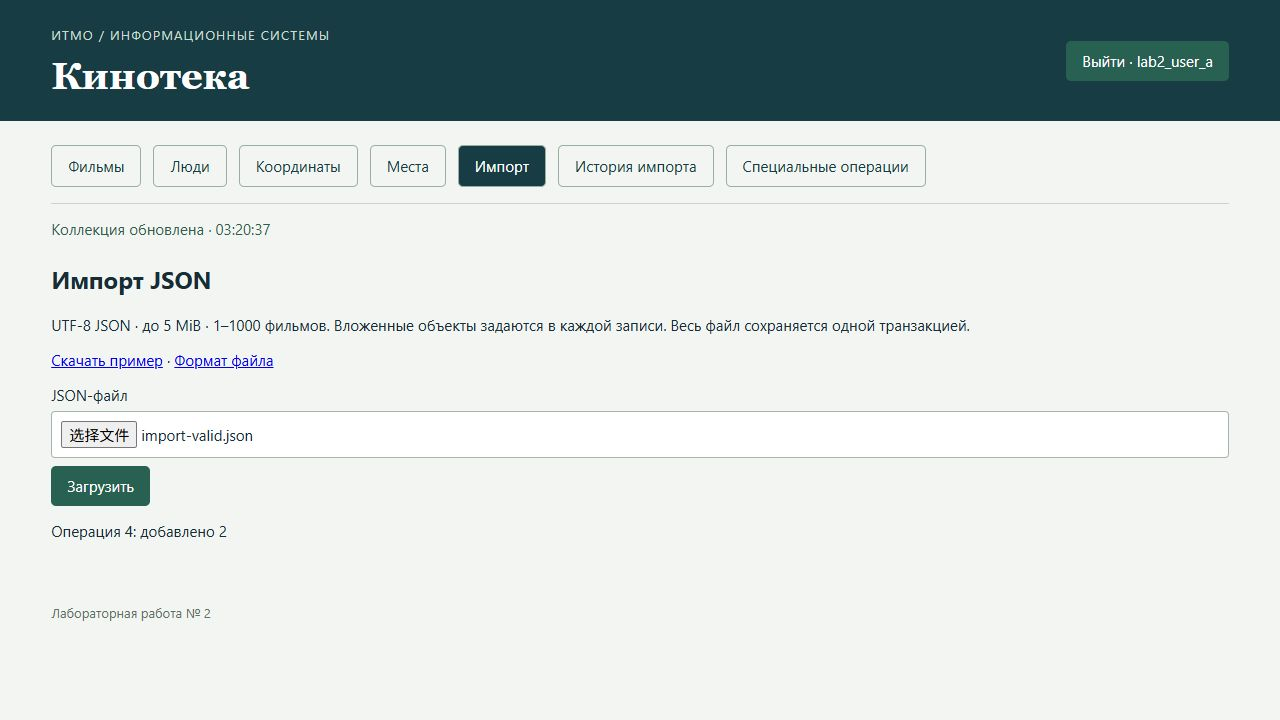
\includegraphics[width=\textwidth]{images/final-import-success.png}
\caption{Загрузка настоящего JSON-файла: два фильма сохранены в формальной установке на Helios}
\end{figure}
\begin{figure}[H]\centering
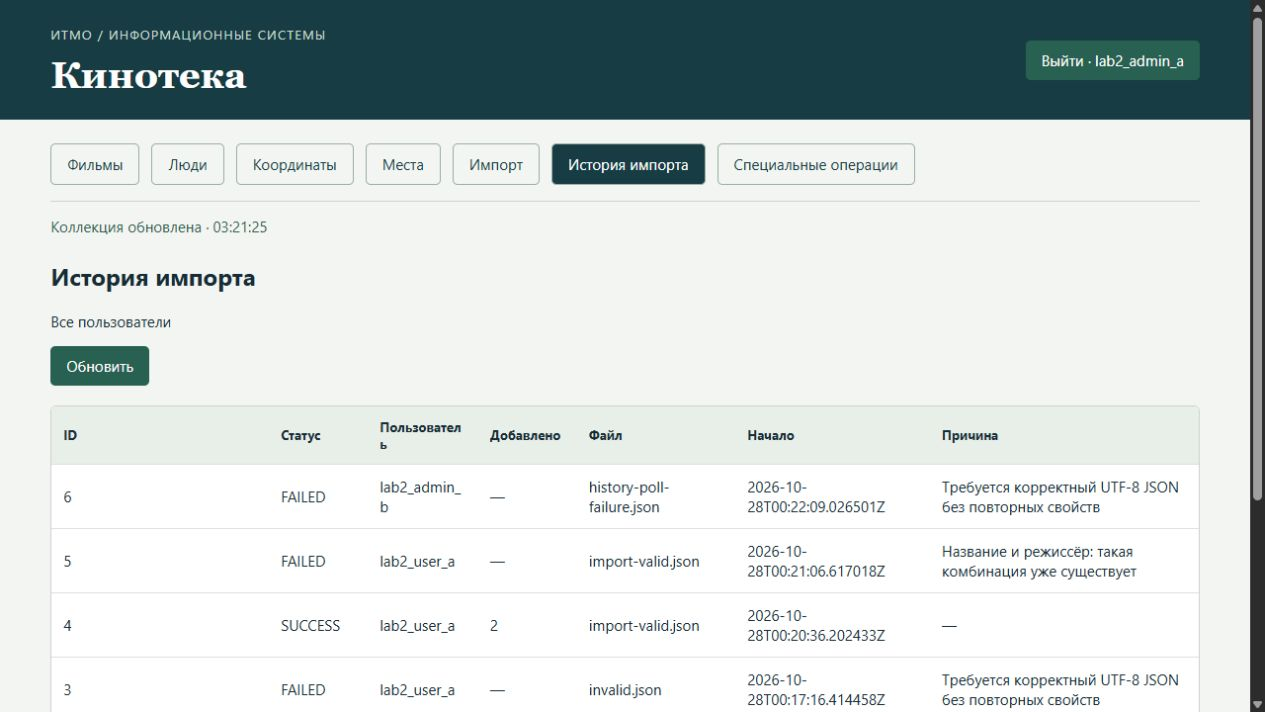
\includegraphics[width=\textwidth]{images/final-history-admin.png}
\caption{Администратор видит операции разных пользователей; FAILED не показывает число объектов}
\end{figure}
\begin{figure}[H]\centering
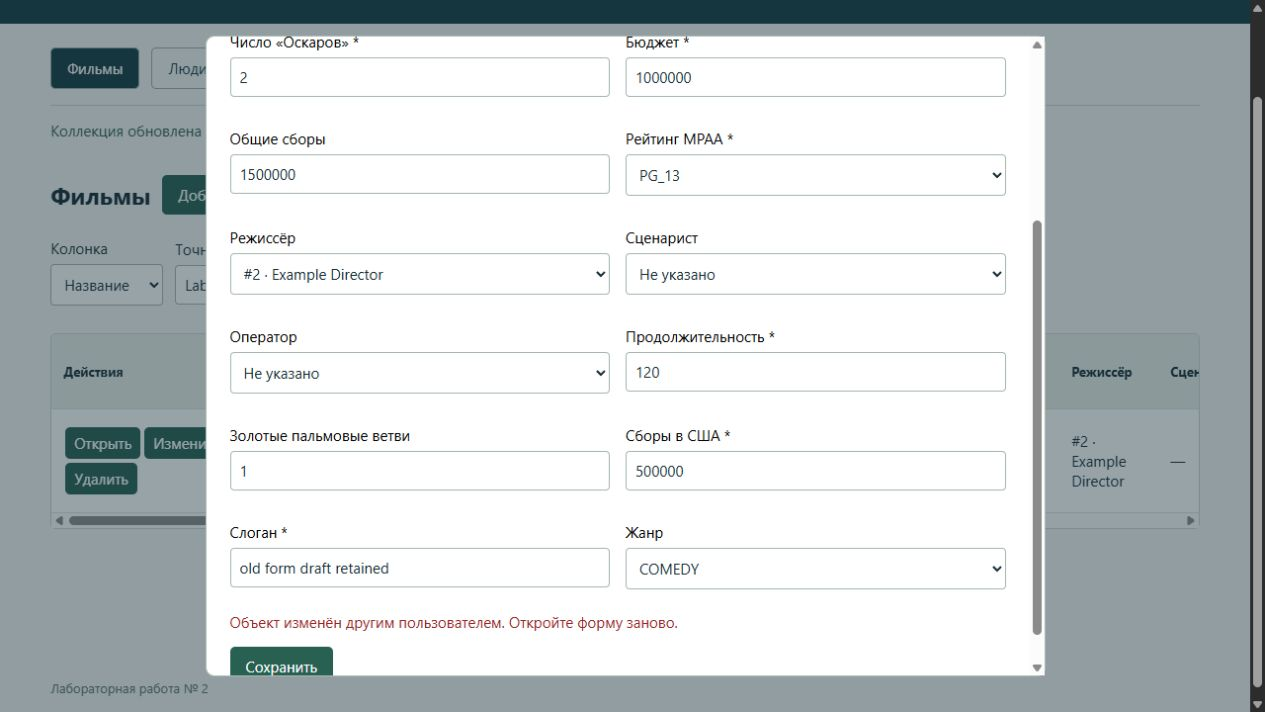
\includegraphics[width=\textwidth]{images/final-stale-edit-conflict.png}
\caption{Старая форма сохраняет черновик и получает конфликт версии вместо перезаписи чужого изменения}
\end{figure}


\subsection{Формальная установка и перезапуск}
Исходный проверенный WAR развёрнут с persistence unit \texttt{movies-helios} на продуктивных таблицах \texttt{lab2\_4101\_}; его SHA-256 совпадает с артефактом обоих окончательных прогонов JMeter. Семнадцать HTTP-проверок повторены на этих таблицах. Прямой снимок PostgreSQL совпадает с объектами API. Хеши исходных таблиц первой работы совпадают с исходным состоянием.

При настоящем перезапуске процесса сохранены четыре проверяемые учётные записи, их роли, фильмы и терминальные записи истории. Отдельная явно созданная SQL-запись RUNNING восстановлена в FAILED; это контрольная запись для проверки recovery, а не утверждение о реально произошедшем неопределённом commit. После обнаруженного выхода прежнего процесса в 05:00 сервис возобновлён тем же WAR; повторно проверены сохранность данных и статусов. Причина выхода из одного журнала приложения не установлена.

После замечаний к интерфейсу на Helios выполнен новый Maven package: изменены четыре веб-файла, остальные записи WAR побайтово совпадают. Выбор файла теперь имеет русские надписи; две подсказки и кнопка обновления удалены. Проверены реальная загрузка, автоматическое появление FAILED без изменения revision и пагинация. Полные JUnit/JMeter повторно не запускались. Доказательства: \path{verification/Lab2/ui-review/} и \path{verification/Lab2/browser/final-ui-checks.json}.

\section{Исходный код и воспроизведение}
Каталог \path{movie-lab/} содержит полный код, миграции, JSON-примеры и JMeter-сценарии. Вместе с отчётом поставляются \href{../../verification/Lab2/source-final.tar.gz}{архив исходников} и \href{../../movie-lab/source-manifest.json}{манифест SHA-256}. Команды воспроизведения приведены в \path{movie-lab/README.md} и \path{movie-lab/jmeter/README.md}, результаты и ограничения --- в \path{verification/Lab2/ACCEPTANCE.md}. JTL, HTML, сырые ответы и снимки БД сохранены для каждого прогона. Пароли, частные дампы и сессионные токены исключены.
